% assignment_2.tex
% CS 8735 - Unsupervised Learning (Fall 2015)
%     University of Missouri-Columbia
%             Chanmann Lim
%            October 2015

\documentclass[a4paper]{article}

\usepackage[margin=1 in]{geometry}
\usepackage{listings}
\usepackage{amsmath}
\usepackage{graphicx}
\usepackage{float}
\usepackage{multirow}

\everymath{\displaystyle}
\DeclareMathOperator*{\argmax}{\arg\!\max}
\DeclareMathOperator*{\argmin}{\arg\!\min}

\begin{document}
\setcounter{page}{6}

\noindent The Matlab code for all experiments is in the \textbf{Appendix} section.

\paragraph{6.} The goal of this problem is to investigate the influences of the ordering of the dataset in sequential clustering algorithm namely \emph{Basic Sequential Algorithmic Scheme (BSAS)} and \emph{Modified Basic Sequential Algorithmic Scheme (MBSAS)}. According to the literature, the main difference between BSAS and MBSAS is that the latter separates the clustering procedure into two parts. Firstly, the class determination phase is served as cluster discovery stage to find out the possible number of clusters with the constraints $\Theta$ : the distance threshold to subsume a data point to a cluster and $q$ : the numbers of maximum allowed clusters. Secondly, the pattern classification stage where each point is being assigned to one of the already created clusters. \\

	\underline{Plot of the vectors:}
	
	\begin{figure}[H]
	  \centering
	    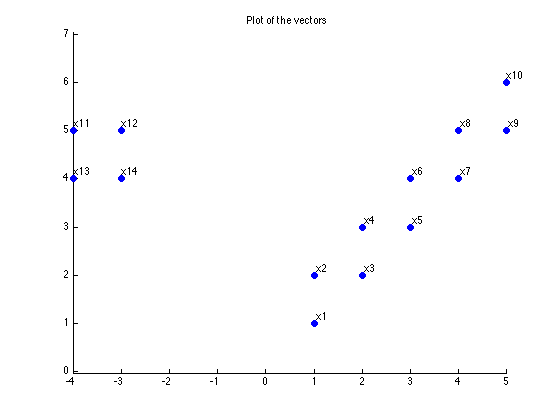
\includegraphics[scale=.57]{images/vectors.png}
	  \caption{Plot of vectors}
	  \label{fig:vectors}
	\end{figure}

	For case \textbf{a.} where the ordering of the dataset is $\mathbf{x}_1, \mathbf{x}_2,\cdots, \mathbf{x}_{14}$ we got:
	
	$$BSAS = \{
		\{ \mathbf{x}_1,  \mathbf{x}_2,  \mathbf{x}_3 \},     
		\{ \mathbf{x}_4,  \mathbf{x}_5,  \mathbf{x}_6 \},     
		\{ \mathbf{x}_7,  \mathbf{x}_8,  \mathbf{x}_9 \},     
		\{ \mathbf{x}_{10} \},     
		\{ \mathbf{x}_{11},  \mathbf{x}_{12},  \mathbf{x}_{13},  \mathbf{x}_{14} \}
	\}$$
	$$MBSAS = \{
		\{ \mathbf{x}_1,  \mathbf{x}_2 \},     
		\{ \mathbf{x}_4,  \mathbf{x}_3,  \mathbf{x}_5 \},     
		\{ \mathbf{x}_7,  \mathbf{x}_6,  \mathbf{x}_8 \},     
		\{ \mathbf{x}_{10},  \mathbf{x}_9 \},     
		\{ \mathbf{x}_{11},  \mathbf{x}_{12},  \mathbf{x}_{13},  \mathbf{x}_{14} \}
	\}$$
	
	\noindent The reason of the difference being MBSAS is trying to balance out the cluster assignment decision until all possible clusters are identified. This solves the problem with BSAS which decided a vector $\mathbf{x}$ to belong to an already created cluster or a new cluster prior to the final cluster formation. \\
	
	For case \textbf{b.} where the ordering of the dataset is $\mathbf{x}_{1},   \mathbf{x}_{10},    \mathbf{x}_{2},    \mathbf{x}_{3},    \mathbf{x}_{4},   \mathbf{x}_{11},   \mathbf{x}_{12},    \mathbf{x}_{5},    \mathbf{x}_{6},    \mathbf{x}_{7},   \mathbf{x}_{13},     \mathbf{x}_{8},   \mathbf{x}_{14},    \mathbf{x}_{9}$ and the clusters obtained:
	
	$$BSAS = \{ \{ \mathbf{x}_{1}, \mathbf{x}_{2}, \mathbf{x}_{3} \},    
		\{ \mathbf{x}_{10}, \mathbf{x}_{9} \},    
		\{ \mathbf{x}_{4}, \mathbf{x}_{5}, \mathbf{x}_{6} \},    
		\{ \mathbf{x}_{11}, \mathbf{x}_{12}, \mathbf{x}_{13}, \mathbf{x}_{14} \},    
		\{ \mathbf{x}_{7}, \mathbf{x}_{8} \} \}$$
	$$MBSAS = \{ \{ \mathbf{x}_{1},  \mathbf{x}_{2} \},    
		\{ \mathbf{x}_{10},  \mathbf{x}_{9} \},    
		\{ \mathbf{x}_{4},  \mathbf{x}_{3},  \mathbf{x}_{5} \},    
		\{ \mathbf{x}_{11},  \mathbf{x}_{12},  \mathbf{x}_{13},  \mathbf{x}_{14} \},    
		\{ \mathbf{x}_{7},  \mathbf{x}_{6},  \mathbf{x}_{8} \} \}$$
		
	For case \textbf{c.} where the ordering of the dataset is $\mathbf{x}_{1},    \mathbf{x}_{10},     \mathbf{x}_{5},     \mathbf{x}_{2},     \mathbf{x}_{3},    \mathbf{x}_{11},    \mathbf{x}_{12},     \mathbf{x}_{4},     \mathbf{x}_{6},     \mathbf{x}_{7},    \mathbf{x}_{13}    \mathbf{x}_{14},     \mathbf{x}_{8},     \mathbf{x}_{9}$ and the clusters obtained:
	
	$$BSAS = \{ \{ \mathbf{x}_{1},  \mathbf{x}_{2},  \mathbf{x}_{3} \},     
		\{ \mathbf{x}_{10},  \mathbf{x}_{9} \},     
		\{ \mathbf{x}_{5},  \mathbf{x}_{4},  \mathbf{x}_{6} \},     
		\{ \mathbf{x}_{11},  \mathbf{x}_{12},  \mathbf{x}_{13},  \mathbf{x}_{14} \},     
		\{ \mathbf{x}_{7},  \mathbf{x}_{8} \} \}$$
	$$MBSAS = \{ \{ \mathbf{x}_{1},  \mathbf{x}_{2},  \mathbf{x}_{3} \},     
		\{ \mathbf{x}_{10},  \mathbf{x}_{8},  \mathbf{x}_{9} \},     
		\{ \mathbf{x}_{5},  \mathbf{x}_{4},  \mathbf{x}_{6},  \mathbf{x}_{7} \},     
		\{ \mathbf{x}_{11},  \mathbf{x}_{12},  \mathbf{x}_{13},  \mathbf{x}_{14} \} \}$$

	\noindent In the last case MBSAS looked through the data and suggested only four clusters conversely BSAS purely depended on the ordering the data set and formed a total of five clusters.

\newpage
\subsection*{Appendix:}
	\lstinputlisting[language=Matlab, title=\lstname, basicstyle=\footnotesize]{assignment_2.m}
	\lstinputlisting[language=Matlab, title=\lstname, basicstyle=\footnotesize]{problem_6.m}
	\lstinputlisting[language=Matlab, title=\lstname, basicstyle=\footnotesize]{bsas.m}
	\lstinputlisting[language=Matlab, title=\lstname, basicstyle=\footnotesize]{mbsas.m}
	\lstinputlisting[language=Matlab, title=\lstname, basicstyle=\footnotesize]{min_distance.m}
	\lstinputlisting[language=Matlab, title=\lstname, basicstyle=\footnotesize]{print_cluster.m}
\end{document}